% mycsrf 'for beeing included' snippet template
%
% (c) Karsten Reincke, Frankfurt a.M. 2012, ff.
%
% This text is licensed under the Creative Commons Attribution 3.0 Germany
% License (http://creativecommons.org/licenses/by/3.0/de/): Feel free to share
% (to copy, distribute and transmit) or to remix (to adapt) it, if you respect
% how you must attribute the work in the manner specified by the author(s):
% \newline
% In an internet based reuse please link the reused parts to mycsrf.fodina.de
% and mention the original author Karsten Reincke in a suitable manner. In a
% paper-like reuse please insert a short hint to mycsrf.fodina.de and to the
% original author, Karsten Reincke, into your preface. For normal quotations
% please use the scientific standard to cite
%


%% use all entries of the bibliography

\subsubsection{NtEd ($\bigstar$$\bigstar$)}
 
Gegenwärtig trifft man im Netz unter dem Stichwort \acc{Notensatzprogramm} auch
noch auf \acc{NtEd}. Die aktuellere Übersicht listet es
ebenso\footcite[vgl.][\nopage wp]{WpedNotensatz2019a}, wie die ältere: dort wird
es unter dem Label \enquote{excellent music notation editor}
präsentiert\footcite[vgl.][\nopage wp]{LinuxSoundNotation2006a}. Über
Distributionen ist das Programm noch zugänglich\footnote{Unter Ubuntu 18.04 mit
\texttt{sudo apt-get install nted}.}. Gleichwohl wird schon darauf hingewiesen,
dass Sourcecode, Projektseite und Handbuch \enquote{seit November 2017} nicht
mehr erreichbar seien\footcite[vgl.][\nopage wp]{UbuntuNtEd2016a}.
Dazu passt, dass selbst der Autor \acc{NtEd} auf seiner
'Selbstvorstellungsseite'\footcite[vgl.][\nopage wp]{Andres2018a} auf eine
\acc{NtEd}-Homepage\footcite[vgl.][\nopage wp]{Andres2018b} verlinkt, die nicht
(mehr) aufgerufen werden kann.
 
Unsere \acc{Referenzkadenz II} kann mit \acc{NtEd} durchaus erfasst werden. Das
Handling ist gelegentlich sperrig\footnote{Um den Bassschlüssel zu aktivieren
muss man 'entdecken', dass ein leerer Mini-Button durch die Alternativen
scrollt.} und 'buggy'\footnote{Nach der Einstellung von 4/2 wurden die ersten
Noten solange über die Schlüssel 'gedruckt', bis wir den Schlüssel noch einmal
zu 4/4 und wieder zurück zu 4/2 gewechselt hatten.}. Nicht alles, was man sehen
möchte\footnote{z.B der Vorhalt in Takt 2 mit einer \Halb gegen 2 \Vier.}, ist
darstellbar. Das 'Druckbild' auf Bildschirm und Papier ist -- verglichen mit
\acc{MusiX\TeX} oder \acc{LilyPond} -- eher unschön. Den Noten kann Text in
einem Lyrikmodus und einem Textmodus zugeordnet werden: Der Lyrikmodus vermag
Wörter resp. Zeichen sogar vertikal auf die Noten auszurichten\footnote{Takt 1}.
Beide Modus können in Grenzen dazu benutzt werden, Harmonieanalysesymbole zu
erfassen; tiefer strukturierte Symbole sind aber nicht darstellbar.

\begin{center}
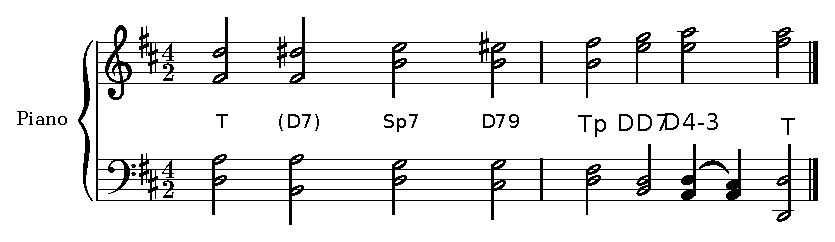
\includegraphics[width=0.8\textwidth]{frontends/nted/candenca2-ntd}
\end{center}

\acc{NtEd} erlaubt den Export im Bild\footnote{PS, PNG, PDF, SVG},
Ton\footnote{Midi}- und \acc{LilyPond}-Format. Der \acc{LilyPond}-Code ist --
sofern man auf textuelle Auszeichnung verzichtet -- klar strukturiert, also zur
Weiterverarbeitung geeignet. Unglücklicherweise scheitert die
Exportverifikation\footnote{$\rightarrow$ S.\pageref{ExportVerifikation}} für
die von NtEd generierte \acc{LilyPond}-Datei; sie enthält eine Klammer zu viel:

\begin{verbatim}
StaffAVoiceA = \relative c' {
   < fis d' >2  < fis dis' >  < b e >  < b f > | % 2
   < b fis' >  < e g >  < e a >  < fis a > 
  \bar "|."
}

StaffA = \new Staff \relative c' {\clef treble\key d \major \time 4/2
  <<
    \new Voice = "one" { \StaffAVoiceA } 
  >>
}

StaffBVoiceA = \relative c' {
   < d, a' >2  < b a' >  < d g >  < cis g' > | % 2
   < d fis >  < b d >  < a d >4 (   < a cis > )   < d, d' >2 
  \bar "|."
}

StaffB = \new Staff \relative c' {\clef bass\key d \major \time 4/2
  <<
    \new Voice = "one" { \StaffBVoiceA } 
  >>
}

\score {
  <<
    \new PianoStaff 
    <<
      \StaffA
%    >> DIESE KLAMMER IST ZUVIEL
      \StaffB
    >>
  >>
  \layout { }
}
\end{verbatim}

Aufs Ganze gesehen wird \acc{NtEd} allenfalls für den Musikwissenschaftler als
'erleichterndes' \acc{LilyPond}-Frontend in Frage kommt, der bereits mit
\acc{NtEd} arbeitet. Sich sein Handling neu anzueignen, ist wenig sinnvoll;
Aufwand, Ergebnis und Wiederverwendbarkeit stehen angesichts des
Entwicklungsstatus nicht im Einklang. Will man als Musikwissenschaftler
\acc{NtEd} dennoch nutzen, kann man darin die Basisversion seines Notentextes
editieren, diese als acc{LilyPond}-Version exportieren und das Ergebnis
anschließend 'manuell' mit einem Texteditor verbessern.

Wir geben dem Programm 2 von 5 Sternen, weil es historisch gesehen durchaus
Verdienste hat und weil es auch heute noch funktioniert.


% this is only inserted to eject fault messages in texlipse
%\bibliography{../bib/literature}
